\documentclass[a4paper, 12pt]{article}

%\usepackage{natbib}
\usepackage[english]{babel}
\usepackage{amsmath, amssymb}
\usepackage{parskip}
\usepackage{graphicx}

\begin{document}

\title{AA2 Practical Assignment}
\author{Maarten de Jonge, Koen Keune, Edwin Odijk,\\ Francesco Stablum, Marysia Winkels}
\maketitle

\section*{Introduction}
%something something sampling based fitted Q-iteration/value-iteration, something something continuous
This report describes the extension on an old AA1 assignment for the AA2 course. The existing predator/prey game's environment was changed from discrete to continuous, and the game was optimized using sampling based fitted Q-iteration/value-iteration.%\cite{ng_lecture}\cite{musze}

\section*{Implementation} 
%HOW IT'S MADE

\section*{Comparison of Algorithms}
%new implementations vs old results
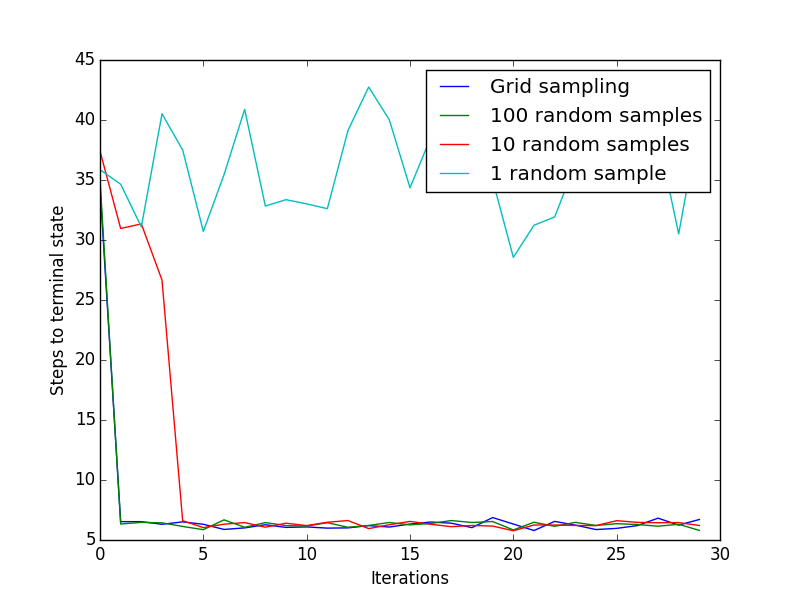
\includegraphics[scale=0.7]{convergence.png}
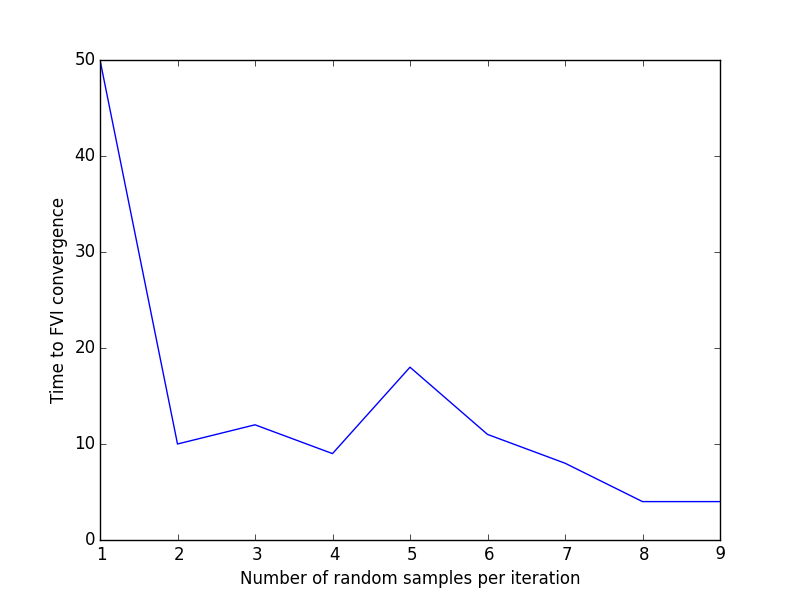
\includegraphics[scale=0.7]{n_samples.png}

\section*{Conclusion}
% ._.

\section*{References}
%\bibliographystyle{plain}
%\bibliography{ref}

\end{document}
